% $Header: /cvsroot/latex-beamer/latex-beamer/solutions/conference-talks/conference-ornate-20min.en.tex,v 1.6 2004/10/07 20:53:08 tantau Exp $

\documentclass{beamer}

% This file is a solution template for:

% - Talk at a conference/colloquium.
% - Talk length is about 20min.
% - Style is ornate.



% Copyright 2004 by Till Tantau <tantau@users.sourceforge.net>.
%
% In principle, this file can be redistributed and/or modified under
% the terms of the GNU Public License, version 2.
%
% However, this file is supposed to be a template to be modified
% for your own needs. For this reason, if you use this file as a
% template and not specifically distribute it as part of a another
% package/program, I grant the extra permission to freely copy and
% modify this file as you see fit and even to delete this copyright
% notice.


\mode<presentation>
{
%  \usetheme{Warsaw}
%  \usetheme{Boadilla}
%  \usetheme{Goettingen}
%  \usetheme{Hannover}
%  \usetheme{Madrid}
%  \usetheme{Marburg}
%  \usetheme{Montpellier}
%  \usetheme{Pittsburgh}
  \usetheme{Hawke}
  % or ...

  \setbeamercovered{transparent}
  % or whatever (possibly just delete it)
}


\usepackage[english]{babel}
% or whatever

\usepackage[latin1]{inputenc}
% or whatever

\usepackage{times}
\usepackage[T1]{fontenc}
% Or whatever. Note that the encoding and the font should match. If T1
% does not look nice, try deleting the line with the fontenc.

\usepackage{multimedia}


%%%%%%
% My Commands
%%%%%%

\newcommand{\ml}{{\sc matlab}}
\newcommand{\bfm}[1]{{\boldsymbol{#1}}}
\newcommand{\bx}{\bfm{x}}
\newcommand{\bb}{\bfm{b}}

%%%%

\title[Lecture 30] % (optional, use only with long paper titles)
{Lecture 30 - Deflation}

% \subtitle
% {Include Only If Paper Has a Subtitle}

\author[I. Hawke] % (optional, use only with lots of authors)
{I.~Hawke}
% - Give the names in the same order as the appear in the paper.
% - Use the \inst{?} command only if the authors have different
%   affiliation.

\institute[University of Southampton] % (optional, but mostly needed)
{
%  \inst{1}%
  School of Mathematics, \\
  University of Southampton, UK
}
% - Use the \inst command only if there are several affiliations.
% - Keep it simple, no one is interested in your street address.

\date[Semester 1] % (optional, should be abbreviation of conference name)
{MATH3018/6141, Semester 1}
% - Either use conference name or its abbreviation.
% - Not really informative to the audience, more for people (including
%   yourself) who are reading the slides online

\subject{Numerical methods}
% This is only inserted into the PDF information catalog. Can be left
% out.



% If you have a file called "university-logo-filename.xxx", where xxx
% is a graphic format that can be processed by latex or pdflatex,
% resp., then you can add a logo as follows:

\pgfdeclareimage[height=0.5cm]{university-logo}{mathematics_7469}
\logo{\pgfuseimage{university-logo}}



% Delete this, if you do not want the table of contents to pop up at
% the beginning of each subsection:
%  \AtBeginSubsection[]
%  {
%    \begin{frame}<beamer>
%      \frametitle{Outline}
%      \tableofcontents[currentsection,currentsubsection]
%    \end{frame}
%  }
\AtBeginSection[]
{
  \begin{frame}<beamer>
    \frametitle{Outline}
    \tableofcontents[currentsection]
  \end{frame}
}


% If you wish to uncover everything in a step-wise fashion, uncomment
% the following command:

%\beamerdefaultoverlayspecification{<+->}


\begin{document}

\begin{frame}
  \titlepage
\end{frame}


\section{Deflation}

\subsection{Deflation}

\begin{frame}
  \frametitle{Nested multiplication}

  When computing the value of a polynomial such as
  \begin{equation*}
    p(z) = a_0 + a_1 z + a_2 z^2 + a_3 z^3
  \end{equation*}
  it is best not to compute the terms individually and add; a huge
  amount of precision is lost. \pause Instead it is usual to write the
  polynomial in nested form
  \begin{equation*}
    p(z) = a_0 + z \left( a_1 + z \left( a_2 + z \left( a_3 \right)
      \right) \right).
  \end{equation*} \pause

  Each individual term is much smaller, so the loss of accuracy due to
  floating point error is greatly reduced.

\end{frame}

\begin{frame}
  \frametitle{The quotient: 1}

  If we wanted to evaluate the nested polynomial of degree $n$
  \begin{equation*}
    p(z) = \sum_{j=0}^n a_j z^j
  \end{equation*}
  at the point $z_0$, we would build the terms
  \begin{align*}
    b_n & = a_n \\
    b_{n-1} & = b_n z_0 + a_{n-1} \\
    \dots \\
    b_0 & = b_1 z_0 + a_0
  \end{align*}
  and note that $p(z_0) = b_0$.

\end{frame}

\begin{frame}
  \frametitle{The quotient: 2}

  Also we can expand the original polynomial as
  \begin{align*}
    p(z) & = \sum_{j=0}^n a_j z^j \\
         & = \sum_{j=0}^{n-1} ( b_{j} - b_{j+1} z_0) z^j + b_n z^n \\
         & = b_0 + b_1 (z - z_0) + b_2 z (z - z_0) + \dots + b_n
         z^{n-1} (z - z_0) \\
         & = b_0 + (z - z_0) \sum_{j=0}^{n-1} b_{j+1} z^{j}.
  \end{align*} \pause
  We define the \emph{quotient} polynomial
  \begin{equation*}
    q(z) = \sum_{j=0}^{n-1} b_{j+1} z^{j}.
  \end{equation*}

\end{frame}

\begin{frame}
  \frametitle{The quotient: 3}

  We have the original polynomial
  \begin{equation*}
    p(z) = (z - z_0) q(z) + b_0
  \end{equation*}
  and $b_0 = p(z_0)$. \pause Therefore if $z_0$ is a root we must have
  $b_0 = 0$ and
  \begin{equation*}
    p(z) = (z - z_0) q(z);
  \end{equation*}
  therefore $q(z)$ describes the behaviour of the polynomial if the
  root is ``divided out''. \pause The quotient is often known as a
  \emph{reduced} or \emph{deflated} polynomial. \pause This deflation
  process can be repeated to find all the roots of the polynomial.
  \pause

  We should note that the build up of errors in the deflation process
  can lead to a completely inaccurate result. Instead of using the
  results as the final word, the deflation method is best used to
  produce accurate initial guesses for Newton's method (applied to the
  full polynomial).

\end{frame}


\subsection{Matrix deflation}

\begin{frame}
  \frametitle{Matrix deflation}

  Deflation is a neat trick for polynomials, but the loss of accuracy
  means that it is still not particularly helpful for computing the
  full spectrum of a matrix direct from the characteristic
  polynomial. \pause

  \vspace{1ex}

  Instead we want to somehow find the ``quotient'' \emph{matrix}; find
  the principal eigenvalue and eigenvector and then ``divide'' this
  out from the matrix. \pause

  \vspace{1ex}

  The question is how to produce a matrix $B$ that contains the
  properties of the original matrix $A$, but not the principal
  eigenvalue and eigenvector.

\end{frame}

\begin{frame}
  \frametitle{Matrix deflation: projection}

  Let us assume that we have the matrix $A$ and have used the power
  method to find the principal eigenvalue $\lambda_1$ with eigenvector
  $\bfm{u}_1$, and sub-principal eigenvalues $\lambda_j$,
  eigenvectors $\bfm{u}_j$, $j>1$. \pause We want to produce a new
  matrix with eigenvalues $\lambda_j$, $j>1$. \pause

  \vspace{1ex}

  If the new matrix $B$ has size $n \times n$ then it must be
  singular. Therefore it will be unsuitable for any method involving
  inversion. However, the power method will still work. Using the new
  matrix $B$, we can construct the sub-principal eigenvalue
  $\lambda_2$, and then iterate down to get all the eigenvalues.
  \pause

  \vspace{1ex}

  So how do we construct the new matrix?

\end{frame}

\begin{frame}
  \frametitle{Matrix deflation: projection 2}

  Given the eigenvalue $\lambda_1$ and eigenvector $\bfm{u}_1$ we can
  build the \emph{projected} matrix
  \begin{equation*}
    B = A - \frac{\lambda_1 \bfm{u}_1 \bfm{u}^{\dagger}_1}{| \bfm{u}_1
      |^2}.
  \end{equation*} \pause

  If we apply this projected matrix to the known eigenvector
  $\bfm{u}_1$ we find
  \begin{align*}
    B \bfm{u}_1 & = A \bfm{u}_1 - \lambda_1 \bfm{u}_1
    \frac{\bfm{u}^{\dagger}_1 \bfm{u}_1}{| \bfm{u}_1 |^2}  \\
    & =  \lambda_1 \bfm{u}_1 -  \lambda_1 \bfm{u}_1 = 0.
  \end{align*} \pause

  Hence if we decompose a general vector in terms of the basis of
  eigenvectors (as in the power method) then the new matrix $B$
  projects out any contribution from the principal eigenvector
  $\bfm{u}_1$.

\end{frame}


\begin{frame}
  \frametitle{Example}


  \begin{columns}
    \begin{column}{0.35\textwidth}
      The matrix
      \begin{equation*}
        A =
        \begin{pmatrix}
          1 & 2 & 3 \\
          4 & 5 & 6 \\
          7 & 8 & 0
        \end{pmatrix}
      \end{equation*}
      has eigenvalues
      \begin{equation*}
        \left\{
          \begin{array}{c}
            12.1229\\ -5.7345\\ -0.3884
          \end{array}\right. .
      \end{equation*}
      The projected deflation algorithm converges to all eigenvalues linearly.
    \end{column}
    \begin{column}{0.65\textwidth}
      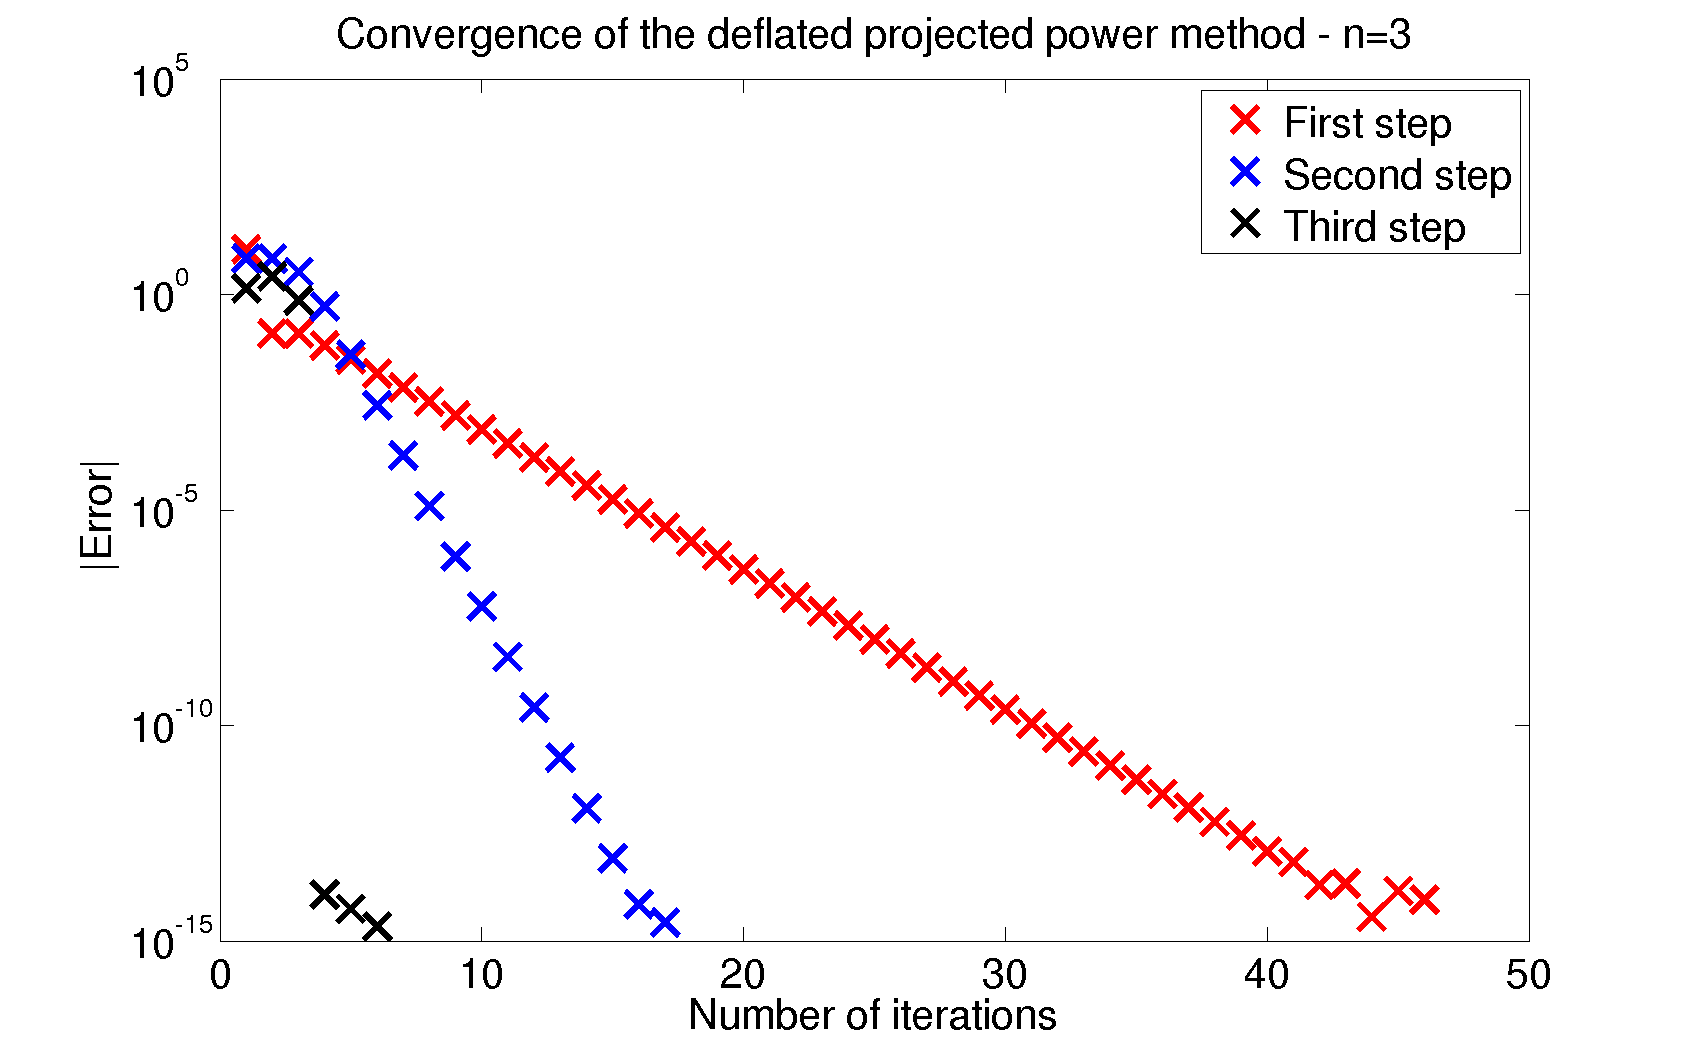
\includegraphics[width=\textwidth]{figures/ProjectionDeflation1}
    \end{column}
  \end{columns}


\end{frame}

\begin{frame}
  \frametitle{Matrix deflation: Householder rotations}

  It turns out that the projection method is not particularly
  stable. This is because the numerical error in determining the
  principal eigenvector means that as the power method is iterated
  this error consistently grows. \pause

  Instead it would be better to construct a smaller $(n - 1) \times (n
  - 1)$ sub-matrix $B$ containing the sub-principal eigenvalues
  $\lambda_j, j>1$. \pause Clearly this matrix $B$ cannot be a simple
  sub-matrix of $A$; instead we have to \emph{rotate} the matrix $A$
  so that the eigenvector we want to remove ($\bfm{u}_1$) is entirely
  contained in one column. \pause

  This would seem an ideal opportunity to use a Householder reflection.
  \pause We know the vector we want to rotate from and to; the (known)
  principle eigenvector $\bfm{u}_1$ and the first unit column vector
  $\bfm{e}_1$.

\end{frame}

\begin{frame}
  \frametitle{Matrix deflation: Householder rotations 2}

  Having constructed the Householder reflection $H$ such that
  \begin{equation*}
    H \bfm{u}_1 = \alpha \bfm{e}_1
  \end{equation*}
  we look at the behaviour of the matrix
  \begin{equation*}
    G = H A H^{\dagger}.
  \end{equation*} \pause
  \begin{overlayarea}{\textwidth}{0.6\textheight}
    \only<2|handout:1>
    {

      As $H$ is unitary by construction we have $H^{\dagger} H =
      \text{Id}$ and hence
      \begin{align*}
        G \left( \alpha \bfm{e}_1 \right) & = G \left( H \bfm{u}_1
        \right)
        \\
        & = H A \left( H^{\dagger} H \right) \bfm{u}_1 \\
        & = H \left( A \bfm{u}_1 \right) \\
        & = \lambda_1 H \bfm{u}_1 \\
        & = \alpha \lambda_1 \bfm{e_1}.
      \end{align*}
    }
    \only<3-|handout:2>
    {
      \begin{equation*}
        G \bfm{e}_1 = \lambda_1 \bfm{e}_1.
      \end{equation*}

      This immediately implies that $\bfm{e}_1$ is the principal
      eigenvector of $G$ and hence $G$ has the form
      \begin{equation*}
        G = \left(
          \begin{array}{c|c}
            \lambda_1 & \bfm{w} \\ \hline
            0 & A_{n-1}
          \end{array}
        \right).
      \end{equation*}
    }
    \only<4|handout:2>
    {
      Therefore from constructing $G$ we have a submatrix $B =
      A_{n-1}$ which has eigenvalues $\lambda_j, j>1$.
    }
  \end{overlayarea}

\end{frame}

\begin{frame}
  \frametitle{Example: 2}


  \begin{columns}
    \begin{column}{0.35\textwidth}
      The matrix
      \begin{equation*}
        A =
        \begin{pmatrix}
          1 & 2 & 3 \\
          4 & 5 & 6 \\
          7 & 8 & 0
        \end{pmatrix}
      \end{equation*}
      has eigenvalues
      \begin{equation*}
        \left\{
          \begin{array}{c}
            12.1229\\ -5.7345\\ -0.3884
          \end{array}\right. .
      \end{equation*}
      The rotated deflation algorithm converges to all eigenvalues linearly.
    \end{column}
    \begin{column}{0.65\textwidth}
      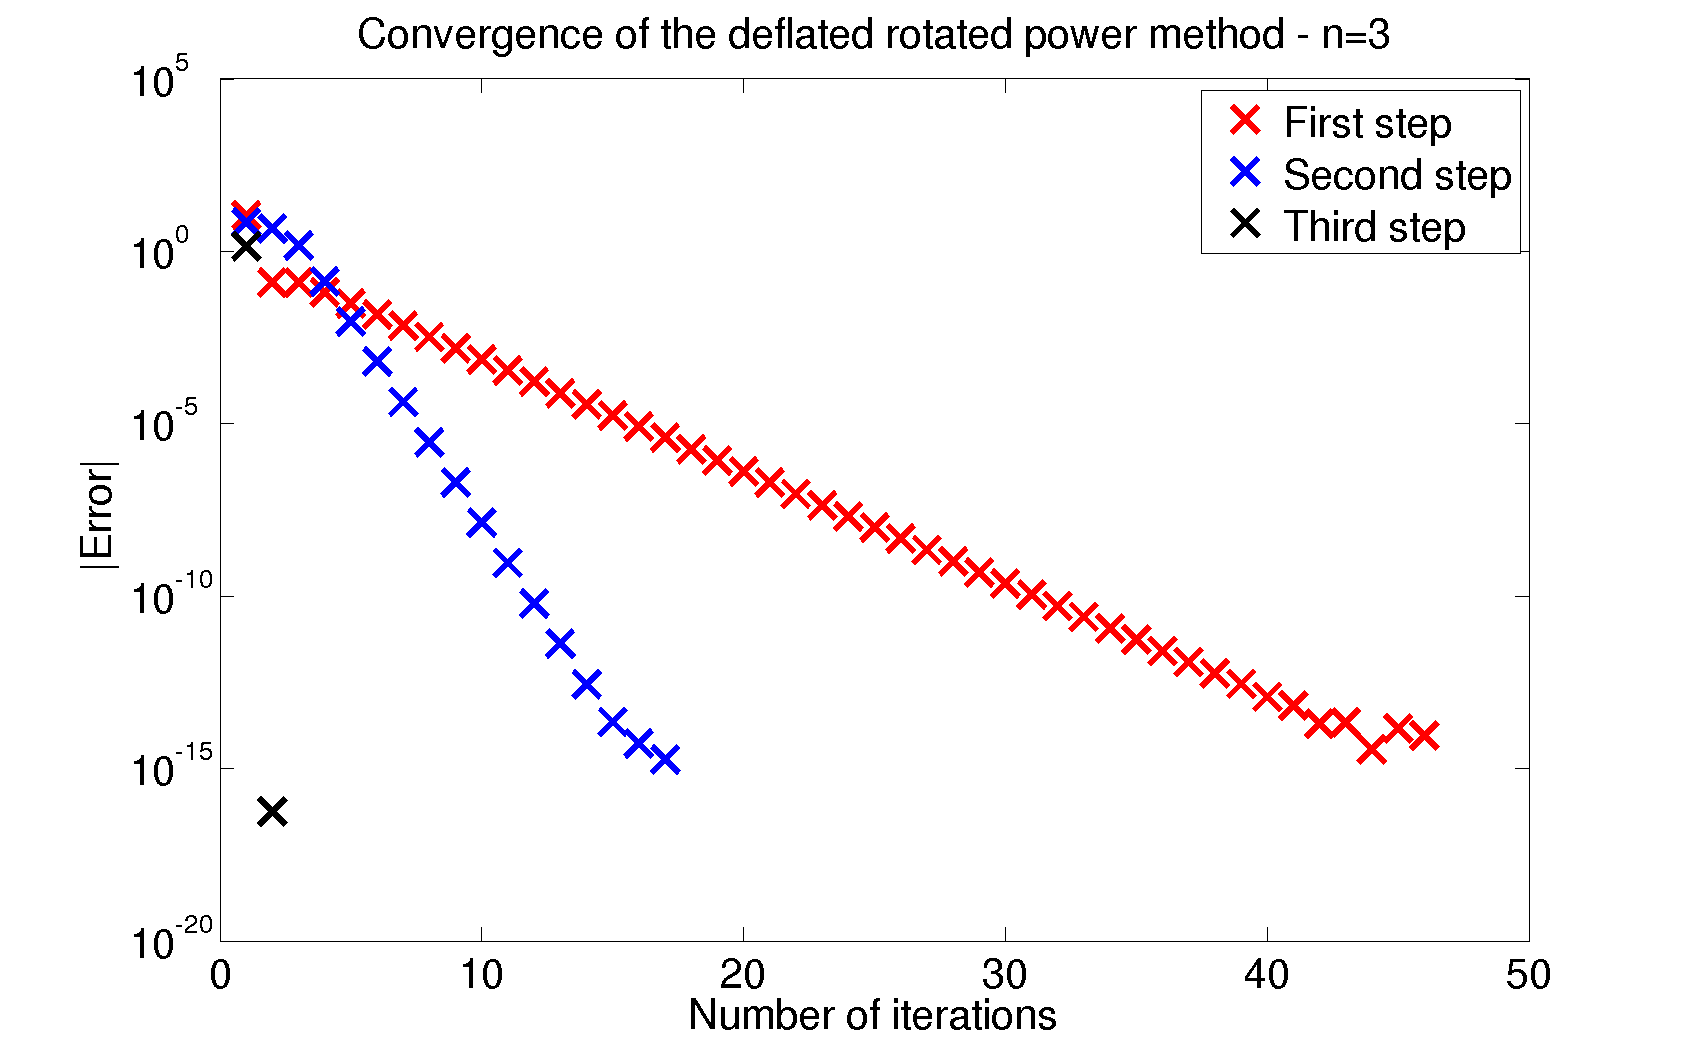
\includegraphics[width=\textwidth]{figures/RotationDeflation1}
    \end{column}
  \end{columns}


\end{frame}

\section{Summary}

\subsection{Summary}

\begin{frame}
  \frametitle{Summary}

  \begin{itemize}
  \item Deflation is a technique to find out the sub-principal
    behaviour of a problem.
  \item For a polynomial problem, we can construct the reduced or
    deflated polynomial by a simple method based on the coefficients
    of the full polynomial.
  \item For a matrix problem we can construct a new matrix with a
    deflated spectrum.
    \begin{enumerate}
    \item The new matrix may have the same size in which case it will
      be singular; by projecting out the principal eigenvector the
      power method works. This method may become unstable.
    \item The new matrix may be smaller; by using a Householder
      reflection the principal eigenvector can be rotated onto the
      first column and the sub-matrix extracted. This method will be
      stable.
    \end{enumerate}
  \item No deflation method can be trusted to give accurate answer for
    large numbers of roots; however, it can be effective for getting
    the leading roots in very large matrices (e.g.\ {\sc pagerank}) or
    for finding initial guesses for other root-finding methods.
  \end{itemize}

\end{frame}

\end{document}



%%% Local Variables:
%%% mode: latex
%%% TeX-master: t
%%% End:
